\documentclass[11pt]{article}
\usepackage[english]{babel}
\usepackage{minted}
\usepackage{amsmath}
\usepackage{graphicx}
\usepackage{float}
\usepackage{xcolor}
\usepackage[left=25mm, top=25mm, bottom=30mm, right=25mm]{geometry}
\usepackage[colorlinks=true, linkcolor=blue, urlcolor=cyan]{hyperref}

\graphicspath{{./figures/}}
\definecolor{mintedbg}{rgb}{0.98,0.97,0.93}

\title{System-Level Temperature-Aware Power Budgeting\\COD494 Progress Report}
\author{Sayam Sethi (2019CS10399)}
\date{May 2023}

\begin{document}

\maketitle

\tableofcontents

\section{Introduction}
This B. Tech. Project II is an extension of the project done in the previous two semesters on ``3D-TemPo: Optimizing 3D DRAM Performance Under Temperature and Power Constraints". The extension involves considering the entire system of memory along with the cores for the optimisation under temperature and power constraints. This is a suitable extension since modern architectures are moving towards an `in-house' design in which the entire system of cores, caches and memory are packaged together and therefore the temperatures of each component greatly affects the other components and since they are packaged together, they would have a combined power budget.

\section{Chosen Architecture}
A HBM2E DRAM having $256$ ranks/banks, across two stacks of $8$ channels has been chosen as the memory, which is the same as the memory architecture that was used for the previous project. For the cores, $8$ cores are chosen which are placed below the memory. Additionally, no caches are used between the cores and the memory. The number of cores is determined in such a way that the dimensions of the $8$ cores, when placed in a $4\times 2$ layout, exactly aligns with the $32$ ranks/banks of the HBM2E memory. This helps to avoid the modelling of the heat transmission via air or a different packaging material which would be required if the dimensions did not align. Additionally, the support for the same is not completely available in the simulator infrastructre (CoMeT) that has been used.\par
The memory would be controlled at a channel level having two states - on or off. In the off state, the channel will not consume any dynamic power and would only consume static power. The cores will be controlled via DVFS. The change in frequency will only affect the dynamic power consumption of the core since the static power is solely temperature dependent.\par
The core-to-channel mapping is not chosen and would be determined as a part of the project in such a way that it incorporates the temperature dependence of vertical neighbours and gives the maximum improvement in the number of epochs it takes to run the benchmarks.

\section{Core-to-Channel Mapping}
We use the fact that maximum temperature dependence is among vertically adjacent neighbours. Additionally, it is optimal to turn on the memory channel and run the core with a non-zero frequency \textit{at the same time}. Otherwise, this would lead to stalling if only the core is on and the memory is off, and would lead to wastage of power when the memory is on and the core is off. Therefore, an optimal mapping would keep channels that are mapped to adjacent cores, vertically adjacent to each other so that the decisions of the adjacency-aware budgeting would align for both memory and cores. Another factor that was taken into account was to map cores on the edges to lower channels since this would more likely distribute the hotspots across the entire system than mapping central cores with lower channels. After using (anti-)symmetry and testing it on small traces, the following core-to-channel mapping was chosen:
\begin{center}
    \begin{tabular}{|c|c|}
        \hline
        Core & Channel\\
        \hline
        0 & 1\\
        1 & 7\\
        2 & 4\\
        3 & 2\\
        4 & 3\\
        5 & 5\\
        6 & 6\\
        7 & 0\\
        \hline
    \end{tabular}
\end{center}

\begin{figure}[H]
    \centering
    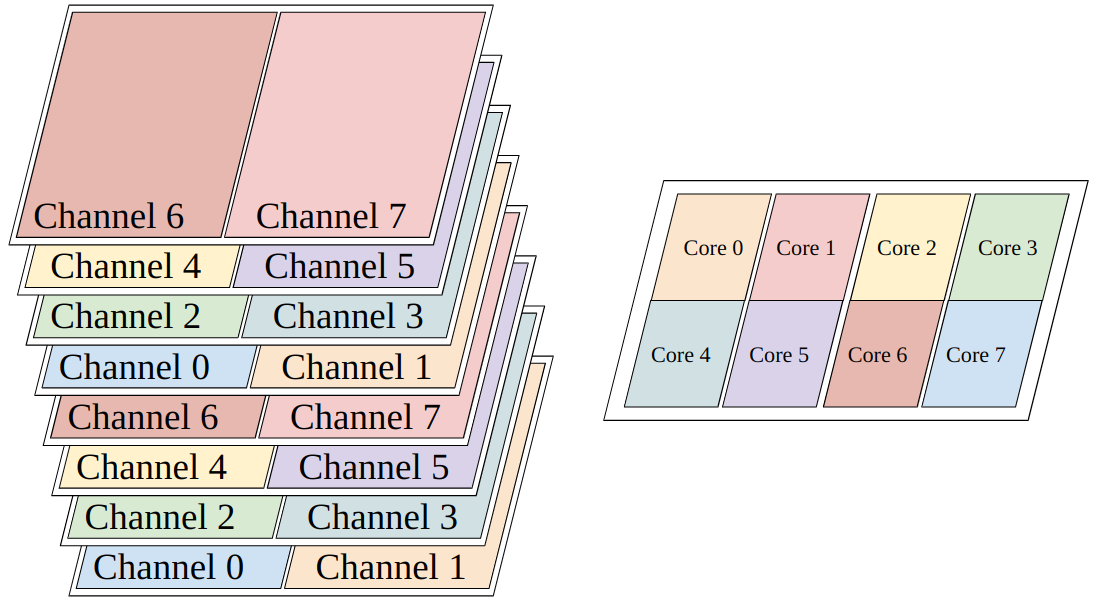
\includegraphics[width=0.75\linewidth]{coretochannel.png}
    \label{fig:ctc}
    \caption{The HBM2E channel layout is shown on the left and the cores layout is shown on the right. The colour scheme is used to indicate the chosen core-to-channel mapping.}
\end{figure}

\section{Proposed Algorithm}
The proposed algorithm is an intuitive extension of the TemPo algorithm that has been used for the 3D-memory power budgeting. Before the algorithm is proposed, some mathematical formulation is given to make it easier to state and explain the algorithm.

\subsection{Mathematical Notation}
We first define the following terms:
\begin{enumerate}
    \item Let the fractional frequency ($=\text{frequency of core}/\text{maximum possible frequency}$) of the core that maps to channel $c$ be denoted by $f_c$.
    \item Let the dynamic power of the channel $c$ be $P_{dyn,c,channel}'$ and that of the core mapped to channel $c$ be $P_{dyn,c,core}'$. Denote the dynamic power that would have been consumed if the core was running at peak frequency as $P_{dyn,c,channel}$ and $P_{dyn,c,core}$. Both of these are just equal to the respective values divided by $f_c$. Let $P_{dyn,c}$ denote the total dynamic power of the core+channel system for channel $c$.
    \item Let the static power of the channel $c$ along with its mapped core be $P_{static,c,0}$ if the channel is off and $P_{static,c,1}$ if the channel is on.
    \item Let the instructions per second of the core corresponding to channel $c$ be $IPC_c'$. If the core runs at peak frequency, let the IPC be denoted as $IPC_c (= IPC_c'/f_c)$.
\end{enumerate}
Now, using the reward function used for TemPo, we get the following reward as a function of the frequency for each core-channel system:
\begin{equation}
    \begin{split}
        R_c(f_c) &= \frac{f_c\cdot IPC_c}{P_{static,c,b} + f_c\cdot P_{dyn,c}}\\
        &=\frac{f_c\cdot \frac{IPC_c}{P_{static,c,b}}}{1 + f_c\cdot P_{dyn,c}/P_{static,c,b}}\\
        &= \frac{f_c\cdot \alpha_{c,b}}{1 + f_c\cdot r_b}\text{, where }\alpha_{c,b} = \frac{IPC_c}{P_{static,c,b}}, r_b = P_{dyn,c}/P_{static,c,b}
    \end{split}
\end{equation}
It is now easy to see that $R_c$ is a monotonic function in $f_c$ and therefore it would have a maxima at $f_c = 1$. This is not a very useful result since this does not help us exploit the potential of performing DVFS on the cores to allow multiple cores to run simultaneously while staying under the power and thermal constraints. The derivative of $R_c$ with respect to $f_c$ is,
\begin{equation}
    \begin{split}
        R_c'(f_c) &= \frac{\alpha_{c,b}}{1 + f_c\cdot r_b} - \frac{f_c\cdot\alpha_{c,b}\cdot r_b}{(1 + f_c\cdot r_b)^2}\\
        &= \frac{\alpha_{c,b}}{(1 + f_c\cdot r_b)^2}
    \end{split}
\end{equation}
Now, this slope is a strictly decreasing function (also apparent from Figure~\ref{fig:rcfc}). Therefore, the change is reward is negligible in comparison to the additional power that is being allocated to the core and channel. Therefore, we can find the maximum frequency value $\hat{f_c}$ for which the slope is at least $1/\beta^2$ for some $\beta > 0$,
\begin{equation}
    \begin{split}
        &\frac{\alpha_{c,b}}{(1 + f_c\cdot r_b)^2} \geq 1/\beta^2\\
        \implies &\frac{\beta\sqrt{\alpha_{c,b}} - 1}{r_b} \geq f_c\\
        \implies &\hat{f_c} = \frac{\beta\sqrt{\alpha_{c,b}} - 1}{r_b}
    \end{split}
\end{equation}

\begin{figure}[H]
    \centering
    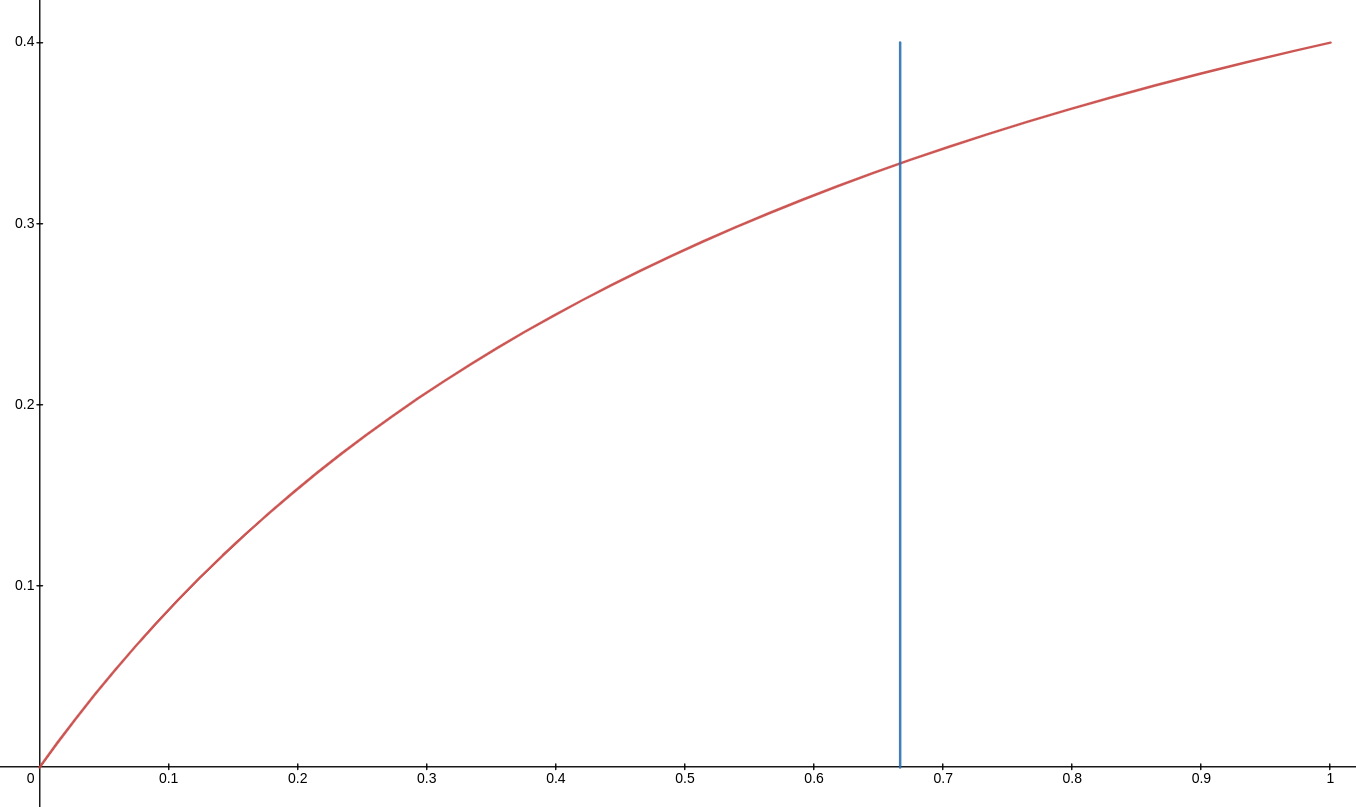
\includegraphics[width=0.75\linewidth]{rcfc.png}
    \label{fig:rcfc}
    \caption{Plot of $R_c$ as a function of $f_c$ for some values of powers and IPC. The vertical line is the value of $\hat{f_c}$ for an arbitrary $\beta$ value}
\end{figure}

Now, the optimal reward that is obtained is,
\begin{equation}
    \begin{split}
        R_c(\hat{f_c}) = \hat{R_c} &= \frac{\frac{\beta\sqrt{\alpha_{c,b}} - 1}{r_b}\cdot\alpha_{c,b}}{1 + \frac{\beta\sqrt{\alpha_{c,b}} - 1}{r_b}\cdot r_b}\\
        &= \frac{\alpha_{c,b}\left(\beta\sqrt{\alpha_{c,b}} - 1\right)}{r_b\cdot\beta\sqrt{\alpha_{c,b}}}\\
        &= \frac{\alpha_{c,b}}{r_b} - \frac{\sqrt{\alpha_{c,b}}}{r_b\cdot\beta}\\
        &= \frac{\sqrt{\alpha_{c,b}}}{r_b}\cdot\left(\sqrt{\alpha_{c,b}} - \frac{1}{\beta}\right)
    \end{split}
\end{equation}

Therefore, this value of $\hat{f_c}$ can be considered a reasonable estimate because of its relation with $\alpha_{c,b}$ and $r_b$. The smaller the $\beta$ we choose, the smaller the value of $\hat{f_c}$ will be and hence we will only increase $f_c$ if there is a significant improvement in the reward function. Additionally, this also takes into account the relation between the static and dynamic power which indirectly incorporates the effects of temperature vs performance via the term $\alpha_{c,b}$. If $\alpha_{c,b}$ is small, then keeping the core on would yield a smaller reward for the same temperature. Similarly, $r_b$ gives an estimate of compute-intensive vs memory-intensive workloads. If the value of $P_{dynamic,c}$ is high, then the number of memory requests are high and therefore the increase in reward will be smaller even on increasing the frequency (as captured via $r_b$). Therefore, we can now extend the TemPo algorithm and determine a suitable value of $\beta$ such that the performance of the system is maximised.

\subsection{Algorithm}
We use the same algorithm as used in the TemPo with slight modifications:
\begin{enumerate}
    \item Instead of computing just one reward function for each channel, we compute two reward functions - one with $b = 0$, one with $b = 1$. The first reward function is considered iff the algorithm determines that the core is compute-intensive (otherwise the core will definitely encounter a memory stall and hence turning on the core without the memory does not make sense)
    \item The reward is computed for the optimal value of frequency $\hat{f_c}(b)$.
\end{enumerate}
Since the core-to-channel mapping has been designed in such a way that vertical neighbours correspond to adjacent cores, the throttling due to vertical neighbours being heated is beneficial even for this algorithm.

\section{Implementation and Pending Work}
\begin{itemize}
    \item Modifications are being made in the CoMeT repository so that it becomes compatible to work with both cores and channels
    \item The implemented algorithm will be run on all the workloads that were used for evaluating TemP
    \item The baseline algorithms would be the same as in the case of TemPo (without any DVFS)
    \item Another baseline algorithm will be used which computes a frequency value to run all cores on such that the total power consumption is within the power budget.
\end{itemize}

\end{document}

